\documentclass[11pt,fleqn]{book}

%%%%%%%%%%%%%%%%%%%%%%%%%%%%%%%%%%%%%%%%%
% The Legrand Orange Book
% Structural Definitions File
% Version 2.0 (9/2/15)
%
% Original author:
% Mathias Legrand (legrand.mathias@gmail.com) with modifications by:
% Vel (vel@latextemplates.com)
% 
% This file has been downloaded from:
% http://www.LaTeXTemplates.com
%
% License:
% CC BY-NC-SA 3.0 (http://creativecommons.org/licenses/by-nc-sa/3.0/)
%
%%%%%%%%%%%%%%%%%%%%%%%%%%%%%%%%%%%%%%%%%

%----------------------------------------------------------------------------------------
%	VARIOUS REQUIRED PACKAGES AND CONFIGURATIONS
%----------------------------------------------------------------------------------------

\usepackage[top=3cm,bottom=3cm,left=3cm,right=3cm,headsep=10pt,a4paper]{geometry} % Page margins

\usepackage{graphicx} % Required for including pictures
\graphicspath{{Pictures/}} % Specifies the directory where pictures are stored

\usepackage{lipsum} % Inserts dummy text

\usepackage{tikz} % Required for drawing custom shapes

\usepackage[english]{babel} % English language/hyphenation

\usepackage{enumitem} % Customize lists
\setlist{nolistsep} % Reduce spacing between bullet points and numbered lists

\usepackage{booktabs} % Required for nicer horizontal rules in tables

\usepackage{xcolor} % Required for specifying colors by name
\definecolor{ocre}{RGB}{243,102,25} % Define the orange color used for highlighting throughout the book

%----------------------------------------------------------------------------------------
%	FONTS
%----------------------------------------------------------------------------------------

\usepackage{avant} % Use the Avantgarde font for headings
%\usepackage{times} % Use the Times font for headings
\usepackage{mathptmx} % Use the Adobe Times Roman as the default text font together with math symbols from the Sym­bol, Chancery and Com­puter Modern fonts

\usepackage{microtype} % Slightly tweak font spacing for aesthetics
\usepackage[utf8]{inputenc} % Required for including letters with accents
\usepackage[T1]{fontenc} % Use 8-bit encoding that has 256 glyphs

%----------------------------------------------------------------------------------------
%	BIBLIOGRAPHY AND INDEX
%----------------------------------------------------------------------------------------

\usepackage[style=alphabetic,citestyle=numeric,sorting=nyt,sortcites=true,autopunct=true,babel=hyphen,hyperref=true,abbreviate=false,backref=true,backend=biber]{biblatex}
\addbibresource{bibliography.bib} % BibTeX bibliography file
\defbibheading{bibempty}{}

\usepackage{calc} % For simpler calculation - used for spacing the index letter headings correctly
\usepackage{makeidx} % Required to make an index
\makeindex % Tells LaTeX to create the files required for indexing

%----------------------------------------------------------------------------------------
%	MAIN TABLE OF CONTENTS
%----------------------------------------------------------------------------------------

\usepackage{titletoc} % Required for manipulating the table of contents

\contentsmargin{0cm} % Removes the default margin

% Part text styling
\titlecontents{part}[0cm]
{\addvspace{20pt}\centering\large\bfseries}
{}
{}
{}

% Chapter text styling
\titlecontents{chapter}[1.25cm] % Indentation
{\addvspace{12pt}\large\sffamily\bfseries} % Spacing and font options for chapters
{\color{ocre!60}\contentslabel[\Large\thecontentslabel]{1.25cm}\color{ocre}} % Chapter number
{\color{ocre}}  
{\color{ocre!60}\normalsize\;\titlerule*[.5pc]{.}\;\thecontentspage} % Page number

% Section text styling
\titlecontents{section}[1.25cm] % Indentation
{\addvspace{3pt}\sffamily\bfseries} % Spacing and font options for sections
{\contentslabel[\thecontentslabel]{1.25cm}} % Section number
{}
{\hfill\color{black}\thecontentspage} % Page number
[]

% Subsection text styling
\titlecontents{subsection}[1.25cm] % Indentation
{\addvspace{1pt}\sffamily\small} % Spacing and font options for subsections
{\contentslabel[\thecontentslabel]{1.25cm}} % Subsection number
{}
{\ \titlerule*[.5pc]{.}\;\thecontentspage} % Page number
[]

% List of figures
\titlecontents{figure}[0em]
{\addvspace{-5pt}\sffamily}
{\thecontentslabel\hspace*{1em}}
{}
{\ \titlerule*[.5pc]{.}\;\thecontentspage}
[]

% List of tables
\titlecontents{table}[0em]
{\addvspace{-5pt}\sffamily}
{\thecontentslabel\hspace*{1em}}
{}
{\ \titlerule*[.5pc]{.}\;\thecontentspage}
[]

%----------------------------------------------------------------------------------------
%	MINI TABLE OF CONTENTS IN PART HEADS
%----------------------------------------------------------------------------------------

% Chapter text styling
\titlecontents{lchapter}[0em] % Indenting
{\addvspace{15pt}\large\sffamily\bfseries} % Spacing and font options for chapters
{\color{ocre}\contentslabel[\Large\thecontentslabel]{1.25cm}\color{ocre}} % Chapter number
{}  
{\color{ocre}\normalsize\sffamily\bfseries\;\titlerule*[.5pc]{.}\;\thecontentspage} % Page number

% Section text styling
\titlecontents{lsection}[0em] % Indenting
{\sffamily\small} % Spacing and font options for sections
{\contentslabel[\thecontentslabel]{1.25cm}} % Section number
{}
{}

% Subsection text styling
\titlecontents{lsubsection}[.5em] % Indentation
{\normalfont\footnotesize\sffamily} % Font settings
{}
{}
{}

%----------------------------------------------------------------------------------------
%	PAGE HEADERS
%----------------------------------------------------------------------------------------

\usepackage{fancyhdr} % Required for header and footer configuration

\pagestyle{fancy}
\renewcommand{\chaptermark}[1]{\markboth{\sffamily\normalsize\bfseries\chaptername\ \thechapter.\ #1}{}} % Chapter text font settings
\renewcommand{\sectionmark}[1]{\markright{\sffamily\normalsize\thesection\hspace{5pt}#1}{}} % Section text font settings
\fancyhf{} \fancyhead[LE,RO]{\sffamily\normalsize\thepage} % Font setting for the page number in the header
\fancyhead[LO]{\rightmark} % Print the nearest section name on the left side of odd pages
\fancyhead[RE]{\leftmark} % Print the current chapter name on the right side of even pages
\renewcommand{\headrulewidth}{0.5pt} % Width of the rule under the header
\addtolength{\headheight}{2.5pt} % Increase the spacing around the header slightly
\renewcommand{\footrulewidth}{0pt} % Removes the rule in the footer
\fancypagestyle{plain}{\fancyhead{}\renewcommand{\headrulewidth}{0pt}} % Style for when a plain pagestyle is specified

% Removes the header from odd empty pages at the end of chapters
\makeatletter
\renewcommand{\cleardoublepage}{
\clearpage\ifodd\c@page\else
\hbox{}
\vspace*{\fill}
\thispagestyle{empty}
\newpage
\fi}

%----------------------------------------------------------------------------------------
%	THEOREM STYLES
%----------------------------------------------------------------------------------------

\usepackage{amsmath,amsfonts,amssymb,amsthm} % For math equations, theorems, symbols, etc

\newcommand{\intoo}[2]{\mathopen{]}#1\,;#2\mathclose{[}}
\newcommand{\ud}{\mathop{\mathrm{{}d}}\mathopen{}}
\newcommand{\intff}[2]{\mathopen{[}#1\,;#2\mathclose{]}}
\newtheorem{notation}{Notation}[chapter]

% Boxed/framed environments
\newtheoremstyle{ocrenumbox}% % Theorem style name
{0pt}% Space above
{0pt}% Space below
{\normalfont}% % Body font
{}% Indent amount
{\small\bf\sffamily\color{ocre}}% % Theorem head font
{\;}% Punctuation after theorem head
{0.25em}% Space after theorem head
{\small\sffamily\color{ocre}\thmname{#1}\nobreakspace\thmnumber{\@ifnotempty{#1}{}\@upn{#2}}% Theorem text (e.g. Theorem 2.1)
\thmnote{\nobreakspace\the\thm@notefont\sffamily\bfseries\color{black}---\nobreakspace#3.}} % Optional theorem note
\renewcommand{\qedsymbol}{$\blacksquare$}% Optional qed square

\newtheoremstyle{blacknumex}% Theorem style name
{5pt}% Space above
{5pt}% Space below
{\normalfont}% Body font
{} % Indent amount
{\small\bf\sffamily}% Theorem head font
{\;}% Punctuation after theorem head
{0.25em}% Space after theorem head
{\small\sffamily{\tiny\ensuremath{\blacksquare}}\nobreakspace\thmname{#1}\nobreakspace\thmnumber{\@ifnotempty{#1}{}\@upn{#2}}% Theorem text (e.g. Theorem 2.1)
\thmnote{\nobreakspace\the\thm@notefont\sffamily\bfseries---\nobreakspace#3.}}% Optional theorem note

\newtheoremstyle{blacknumbox} % Theorem style name
{0pt}% Space above
{0pt}% Space below
{\normalfont}% Body font
{}% Indent amount
{\small\bf\sffamily}% Theorem head font
{\;}% Punctuation after theorem head
{0.25em}% Space after theorem head
{\small\sffamily\thmname{#1}\nobreakspace\thmnumber{\@ifnotempty{#1}{}\@upn{#2}}% Theorem text (e.g. Theorem 2.1)
\thmnote{\nobreakspace\the\thm@notefont\sffamily\bfseries---\nobreakspace#3.}}% Optional theorem note

% Non-boxed/non-framed environments
\newtheoremstyle{ocrenum}% % Theorem style name
{5pt}% Space above
{5pt}% Space below
{\normalfont}% % Body font
{}% Indent amount
{\small\bf\sffamily\color{ocre}}% % Theorem head font
{\;}% Punctuation after theorem head
{0.25em}% Space after theorem head
{\small\sffamily\color{ocre}\thmname{#1}\nobreakspace\thmnumber{\@ifnotempty{#1}{}\@upn{#2}}% Theorem text (e.g. Theorem 2.1)
\thmnote{\nobreakspace\the\thm@notefont\sffamily\bfseries\color{black}---\nobreakspace#3.}} % Optional theorem note
\renewcommand{\qedsymbol}{$\blacksquare$}% Optional qed square
\makeatother

% Defines the theorem text style for each type of theorem to one of the three styles above
\newcounter{dummy} 
\numberwithin{dummy}{section}
\theoremstyle{ocrenumbox}
\newtheorem{theoremeT}[dummy]{Theorem}
\newtheorem{problem}{Problem}[chapter]
\newtheorem{exerciseT}{Exercise}[chapter]
\theoremstyle{blacknumex}
\newtheorem{exampleT}{Example}[chapter]
\theoremstyle{blacknumbox}
\newtheorem{vocabulary}{Vocabulary}[chapter]
\newtheorem{definitionT}{Definition}[section]
\newtheorem{corollaryT}[dummy]{Corollary}
\theoremstyle{ocrenum}
\newtheorem{proposition}[dummy]{Proposition}

%----------------------------------------------------------------------------------------
%	DEFINITION OF COLORED BOXES
%----------------------------------------------------------------------------------------

\RequirePackage[framemethod=default]{mdframed} % Required for creating the theorem, definition, exercise and corollary boxes

% Theorem box
\newmdenv[skipabove=7pt,
skipbelow=7pt,
backgroundcolor=black!5,
linecolor=ocre,
innerleftmargin=5pt,
innerrightmargin=5pt,
innertopmargin=5pt,
leftmargin=0cm,
rightmargin=0cm,
innerbottommargin=5pt]{tBox}

% Exercise box	  
\newmdenv[skipabove=7pt,
skipbelow=7pt,
rightline=false,
leftline=true,
topline=false,
bottomline=false,
backgroundcolor=ocre!10,
linecolor=ocre,
innerleftmargin=5pt,
innerrightmargin=5pt,
innertopmargin=5pt,
innerbottommargin=5pt,
leftmargin=0cm,
rightmargin=0cm,
linewidth=4pt]{eBox}	

% Definition box
\newmdenv[skipabove=7pt,
skipbelow=7pt,
rightline=false,
leftline=true,
topline=false,
bottomline=false,
linecolor=ocre,
innerleftmargin=5pt,
innerrightmargin=5pt,
innertopmargin=0pt,
leftmargin=0cm,
rightmargin=0cm,
linewidth=4pt,
innerbottommargin=0pt]{dBox}	

% Corollary box
\newmdenv[skipabove=7pt,
skipbelow=7pt,
rightline=false,
leftline=true,
topline=false,
bottomline=false,
linecolor=gray,
backgroundcolor=black!5,
innerleftmargin=5pt,
innerrightmargin=5pt,
innertopmargin=5pt,
leftmargin=0cm,
rightmargin=0cm,
linewidth=4pt,
innerbottommargin=5pt]{cBox}

% Creates an environment for each type of theorem and assigns it a theorem text style from the "Theorem Styles" section above and a colored box from above
\newenvironment{theorem}{\begin{tBox}\begin{theoremeT}}{\end{theoremeT}\end{tBox}}
\newenvironment{exercise}{\begin{eBox}\begin{exerciseT}}{\hfill{\color{ocre}\tiny\ensuremath{\blacksquare}}\end{exerciseT}\end{eBox}}				  
\newenvironment{definition}{\begin{dBox}\begin{definitionT}}{\end{definitionT}\end{dBox}}	
\newenvironment{example}{\begin{exampleT}}{\hfill{\tiny\ensuremath{\blacksquare}}\end{exampleT}}		
\newenvironment{corollary}{\begin{cBox}\begin{corollaryT}}{\end{corollaryT}\end{cBox}}	

%----------------------------------------------------------------------------------------
%	REMARK ENVIRONMENT
%----------------------------------------------------------------------------------------

\newenvironment{remark}{\par\vspace{10pt}\small % Vertical white space above the remark and smaller font size
\begin{list}{}{
\leftmargin=35pt % Indentation on the left
\rightmargin=25pt}\item\ignorespaces % Indentation on the right
\makebox[-2.5pt]{\begin{tikzpicture}[overlay]
\node[draw=ocre!60,line width=1pt,circle,fill=ocre!25,font=\sffamily\bfseries,inner sep=2pt,outer sep=0pt] at (-15pt,0pt){\textcolor{ocre}{R}};\end{tikzpicture}} % Orange R in a circle
\advance\baselineskip -1pt}{\end{list}\vskip5pt} % Tighter line spacing and white space after remark

%----------------------------------------------------------------------------------------
%	SECTION NUMBERING IN THE MARGIN
%----------------------------------------------------------------------------------------

\makeatletter
\renewcommand{\@seccntformat}[1]{\llap{\textcolor{ocre}{\csname the#1\endcsname}\hspace{1em}}}                    
\renewcommand{\section}{\@startsection{section}{1}{\z@}
{-4ex \@plus -1ex \@minus -.4ex}
{1ex \@plus.2ex }
{\normalfont\large\sffamily\bfseries}}
\renewcommand{\subsection}{\@startsection {subsection}{2}{\z@}
{-3ex \@plus -0.1ex \@minus -.4ex}
{0.5ex \@plus.2ex }
{\normalfont\sffamily\bfseries}}
\renewcommand{\subsubsection}{\@startsection {subsubsection}{3}{\z@}
{-2ex \@plus -0.1ex \@minus -.2ex}
{.2ex \@plus.2ex }
{\normalfont\small\sffamily\bfseries}}                        
\renewcommand\paragraph{\@startsection{paragraph}{4}{\z@}
{-2ex \@plus-.2ex \@minus .2ex}
{.1ex}
{\normalfont\small\sffamily\bfseries}}

%----------------------------------------------------------------------------------------
%	PART HEADINGS
%----------------------------------------------------------------------------------------

% numbered part in the table of contents
\newcommand{\@mypartnumtocformat}[2]{%
\setlength\fboxsep{0pt}%
\noindent\colorbox{ocre!20}{\strut\parbox[c][.7cm]{\ecart}{\color{ocre!70}\Large\sffamily\bfseries\centering#1}}\hskip\esp\colorbox{ocre!40}{\strut\parbox[c][.7cm]{\linewidth-\ecart-\esp}{\Large\sffamily\centering#2}}}%
%%%%%%%%%%%%%%%%%%%%%%%%%%%%%%%%%%
% unnumbered part in the table of contents
\newcommand{\@myparttocformat}[1]{%
\setlength\fboxsep{0pt}%
\noindent\colorbox{ocre!40}{\strut\parbox[c][.7cm]{\linewidth}{\Large\sffamily\centering#1}}}%
%%%%%%%%%%%%%%%%%%%%%%%%%%%%%%%%%%
\newlength\esp
\setlength\esp{4pt}
\newlength\ecart
\setlength\ecart{1.2cm-\esp}
\newcommand{\thepartimage}{}%
\newcommand{\partimage}[1]{\renewcommand{\thepartimage}{#1}}%
\def\@part[#1]#2{%
\ifnum \c@secnumdepth >-2\relax%
\refstepcounter{part}%
\addcontentsline{toc}{part}{\texorpdfstring{\protect\@mypartnumtocformat{\thepart}{#1}}{\partname~\thepart\ ---\ #1}}
\else%
\addcontentsline{toc}{part}{\texorpdfstring{\protect\@myparttocformat{#1}}{#1}}%
\fi%
\startcontents%
\markboth{}{}%
{\thispagestyle{empty}%
\begin{tikzpicture}[remember picture,overlay]%
\node at (current page.north west){\begin{tikzpicture}[remember picture,overlay]%	
\fill[ocre!20](0cm,0cm) rectangle (\paperwidth,-\paperheight);
\node[anchor=north] at (4cm,-3.25cm){\color{ocre!40}\fontsize{220}{100}\sffamily\bfseries\@Roman\c@part}; 
\node[anchor=south east] at (\paperwidth-1cm,-\paperheight+1cm){\parbox[t][][t]{8.5cm}{
\printcontents{l}{0}{\setcounter{tocdepth}{1}}%
}};
\node[anchor=north east] at (\paperwidth-1.5cm,-3.25cm){\parbox[t][][t]{15cm}{\strut\raggedleft\color{white}\fontsize{30}{30}\sffamily\bfseries#2}};
\end{tikzpicture}};
\end{tikzpicture}}%
\@endpart}
\def\@spart#1{%
\startcontents%
\phantomsection
{\thispagestyle{empty}%
\begin{tikzpicture}[remember picture,overlay]%
\node at (current page.north west){\begin{tikzpicture}[remember picture,overlay]%	
\fill[ocre!20](0cm,0cm) rectangle (\paperwidth,-\paperheight);
\node[anchor=north east] at (\paperwidth-1.5cm,-3.25cm){\parbox[t][][t]{15cm}{\strut\raggedleft\color{white}\fontsize{30}{30}\sffamily\bfseries#1}};
\end{tikzpicture}};
\end{tikzpicture}}
\addcontentsline{toc}{part}{\texorpdfstring{%
\setlength\fboxsep{0pt}%
\noindent\protect\colorbox{ocre!40}{\strut\protect\parbox[c][.7cm]{\linewidth}{\Large\sffamily\protect\centering #1\quad\mbox{}}}}{#1}}%
\@endpart}
\def\@endpart{\vfil\newpage
\if@twoside
\if@openright
\null
\thispagestyle{empty}%
\newpage
\fi
\fi
\if@tempswa
\twocolumn
\fi}

%----------------------------------------------------------------------------------------
%	CHAPTER HEADINGS
%----------------------------------------------------------------------------------------

\newcommand{\thechapterimage}{}%
\newcommand{\chapterimage}[1]{\renewcommand{\thechapterimage}{#1}}%
\def\@makechapterhead#1{%
{\parindent \z@ \raggedright \normalfont
\ifnum \c@secnumdepth >\m@ne
\if@mainmatter
\begin{tikzpicture}[remember picture,overlay]
\node at (current page.north west)
{\begin{tikzpicture}[remember picture,overlay]
\node[anchor=north west,inner sep=0pt] at (0,0) {\includegraphics[width=\paperwidth]{\thechapterimage}};
\draw[anchor=west] (\Gm@lmargin,-9cm) node [line width=2pt,rounded corners=15pt,draw=ocre,fill=white,fill opacity=0.5,inner sep=15pt]{\strut\makebox[22cm]{}};
\draw[anchor=west] (\Gm@lmargin+.3cm,-9cm) node {\huge\sffamily\bfseries\color{black}\thechapter. #1\strut};
\end{tikzpicture}};
\end{tikzpicture}
\else
\begin{tikzpicture}[remember picture,overlay]
\node at (current page.north west)
{\begin{tikzpicture}[remember picture,overlay]
\node[anchor=north west,inner sep=0pt] at (0,0) {\includegraphics[width=\paperwidth]{\thechapterimage}};
\draw[anchor=west] (\Gm@lmargin,-9cm) node [line width=2pt,rounded corners=15pt,draw=ocre,fill=white,fill opacity=0.5,inner sep=15pt]{\strut\makebox[22cm]{}};
\draw[anchor=west] (\Gm@lmargin+.3cm,-9cm) node {\huge\sffamily\bfseries\color{black}#1\strut};
\end{tikzpicture}};
\end{tikzpicture}
\fi\fi\par\vspace*{270\p@}}}

%-------------------------------------------

\def\@makeschapterhead#1{%
\begin{tikzpicture}[remember picture,overlay]
\node at (current page.north west)
{\begin{tikzpicture}[remember picture,overlay]
\node[anchor=north west,inner sep=0pt] at (0,0) {\includegraphics[width=\paperwidth]{\thechapterimage}};
\draw[anchor=west] (\Gm@lmargin,-9cm) node [line width=2pt,rounded corners=15pt,draw=ocre,fill=white,fill opacity=0.5,inner sep=15pt]{\strut\makebox[22cm]{}};
\draw[anchor=west] (\Gm@lmargin+.3cm,-9cm) node {\huge\sffamily\bfseries\color{black}#1\strut};
\end{tikzpicture}};
\end{tikzpicture}
\par\vspace*{270\p@}}
\makeatother

%----------------------------------------------------------------------------------------
%	HYPERLINKS IN THE DOCUMENTS
%----------------------------------------------------------------------------------------

\usepackage{hyperref}
\hypersetup{hidelinks,backref=true,pagebackref=true,hyperindex=true,colorlinks=false,breaklinks=true,urlcolor= ocre,bookmarks=true,bookmarksopen=false,pdftitle={Title},pdfauthor={Author}}
\usepackage{bookmark}
\bookmarksetup{
open,
numbered,
addtohook={%
\ifnum\bookmarkget{level}=0 % chapter
\bookmarksetup{bold}%
\fi
\ifnum\bookmarkget{level}=-1 % part
\bookmarksetup{color=ocre,bold}%
\fi
}
} 
\usepackage{minted}
\usepackage{parskip}
\usepackage{amsmath}
\usepackage{listings}

\newcommand{\argmin}{\arg\!\min}
\newcommand{\argmax}{\arg\!\max}
\newcommand{\myheader}[1]{\textbf{#1 } \hspace{0.2cm}}

\newcommand{\myequ}[1]{\begin{align}\begin{split} #1 \end{split}\end{align}}

\definecolor{mygray}{rgb}{0.5,0.5,0.5}
\definecolor{mymauve}{rgb}{0.58,0,0.82}
\lstdefinestyle{liststy}{
	mathescape,
	columns=fullflexible,
	basicstyle=\fontfamily{lmvtt}\selectfont,
	frame=L,
	xleftmargin=\parindent,
	tabsize=4,
	frame=single,
	numberstyle=\tiny\color{mygray},
	numbers=left,
}



\usepackage{fontspec}

\setsansfont{Calibri}
\setmonofont{Consolas}

\newminted{haskell}{
    frame=single,framesep=10pt,
    mathescape,
    linenos,
    numbersep=5pt,
    breaklines,
    breakautoindent=false,
    breaksymbolleft=\raisebox{0.8ex}{
        \small\reflectbox{\carriagereturn}},
    breaksymbolindentleft=0pt,
    breaksymbolsepleft=0pt,
    breaksymbolright=\small\carriagereturn,
    breaksymbolindentright=0pt,
    breaksymbolsepright=0pt,
    }
\renewcommand{\theFancyVerbLine}{
\sffamily\textcolor[rgb]{0.5,0.5,0.5}{\scriptsize\arabic{FancyVerbLine}}}

\begin{document}
	\begingroup
	\thispagestyle{empty}
	\begin{tikzpicture}[remember picture,overlay]
	\coordinate [below=12cm] (midpoint) at (current page.north);
	\node at (current page.north west)
	{\begin{tikzpicture}[remember picture,overlay]
		\node[anchor=north west,inner sep=0pt] at (0,0) {
\includegraphics[width=\paperwidth]{background}}; 
		\draw[anchor=north] (midpoint) node [fill=ocre!30!white,fill opacity=0.6,text opacity=1,inner sep=1cm]{\Huge\centering\bfseries\sffamily\parbox[c][][t]{\paperwidth}{\centering Daily Notes\\[15pt] % Book title
				{\Large Keep Moving, Never Stop}\\[20pt] % Subtitle
				{\huge Sai Bi}}}; % Author name
		\end{tikzpicture}};
\end{tikzpicture}
\vfill
\endgroup

\newpage
~\vfill
\thispagestyle{empty}

\noindent Copyright \copyright\ 2016  Sai Bi\\ 

\noindent Licensed under the Creative Commons Attribution-NonCommercial 3.0 Unported License (the ``License''). You may not use this file except in compliance with the License. You may obtain a copy of the License at \url{http://creativecommons.org/licenses/by-nc/3.0}. Unless required by applicable law or agreed to in writing, software distributed under the License is distributed on an \textsc{``as is'' basis, without warranties or conditions of any kind}, either express or implied. See the License for the specific language governing permissions and limitations under the License.\\ % License information

\noindent \textit{Start from January 2016} % Printing/edition date

\chapterimage{chapter_head_1.pdf} 

\pagestyle{empty} 
\cleardoublepage
\pagestyle{fancy}


\part{Year 2016}

\chapterimage{chapter_head_2.pdf}

% \chapter{February}

\section{Feb 1st}\index{Feb 1st}
\subsection{Standard deviation} \index{Standard deviation}
\textbf{Standard deviation} $\sigma$ is defined as the square root of \textbf{variance}. That is,
\begin{align}
	\sigma(X) &= \sqrt{var(X)}
\end{align}
The definition for variance:
\begin{align}
var(X) = E[(X - \mu_X)^2]
\end{align}
The definition for \textbf{covariance}:
\begin{align}
cov(X,Y) = E[(X - \mu_X)(Y- \mu_Y)]
\end{align}
A property:
\begin{align}
	cov(X,X) = var(X) = \sigma(X)^2 
\end{align}
Definition for \textbf{correlation}:
\begin{align}
	\begin{split}
	\rho(X,Y) & = corr(X, Y) 		\\
			  & = \frac{cov(X,Y)}{\sigma_X \sigma_Y}
	\end{split}
\end{align}

\section{Feb 2nd}\index{Feb 2nd}

\subsection{Determinant}\index{Determinant}
Today when I try to compute the determinant of the covariance matrix in the multivariate Gaussian, I come across the problem of overflow. In fact, I only
need to know the logarithm of the determinant. Therefore, I apply the following solution:
\begin{align}
	\begin{split}
	\log(\det A) &= \log(\Pi_{i=1}^{N} \lambda_i)  \\
				 & = \sum_{i=1}^{N} \log(\lambda_i)
	\end{split}
\end{align}

\subsection{Matplotlib}\index{Matplotlib}
Sample code to plot figures with Python:

\begin{minted}[frame=lines, framesep=2mm,]
	       {python}
x = np.linspace(-10, 4, 500, endpoint=True)
y = (3 * x + 12) / 4

fig = plt.figure()
fig.suptitle('Problem 3', fontsize=20, fontweight='bold')
ax = fig.add_subplot(111)
ax.plot(x, y)

ax.spines['right'].set_color('none')
ax.spines['top'].set_color('none')
ax.xaxis.set_ticks_position('bottom')
ax.spines['bottom'].set_position(('data',0))
ax.yaxis.set_ticks_position('left')
ax.spines['left'].set_position(('data',0))

plt.annotate(r'$(-4,0)$',
xy=(-4, 0), xycoords='data',
xytext=(-20, +60), textcoords='offset points', fontsize=16,
arrowprops=dict(arrowstyle="->", connectionstyle="arc3,rad=.2"))

plt.annotate(r'$(0,3)$',
xy=(0, 3), xycoords='data',
xytext=(+10, -30), textcoords='offset points', fontsize=16,
arrowprops=dict(arrowstyle="->", connectionstyle="arc3,rad=.2"))

plt.annotate(r'positive',
xy=(-6, 2), xycoords='data',
xytext=(+10, +30), textcoords='offset points', fontsize=16)

ax.set_xlabel("x")
ax.set_ylabel("y")

plt.savefig('3.png', dpi = 100)
plt.show()
\end{minted}

\section{Feb 3rd}\index{Feb 2nd}
\subsection{Different types of machine learning methods:}
\begin{enumerate}
\item \textbf{Parametric methods}: a family of distributions that can be described using a finite 
number of paramters, such as \textit{GMM, Naive Bayes, SVM}.
\item \textbf{Non-parametric methods}: methods that are not based on parametrized families of
probability distributions, such as \textit{decision trees, KNN}. 
\end{enumerate}

The difference between parametric models and non-parametric models is that the former 
has a fixed number of parameters, while the latter grows the number of parameters with 
the amount of training data.
\begin{remark}
Note that the non-parametric model does not have no parameters: parameters are determined by the training data, not the model.
\end{remark}

Parametric models can also be categorized into \textbf{generative models} and 
\textbf{discriminative models}.
\begin{enumerate}
\item Generative models: Fit a probability distribution like a multivariate Gaussian to each class.
\item Approximate the boundaries between classes by simple functions.
\end{enumerate}

\subsection{Representation Learning}


\paragraph{Dimensionality Reduction and Denoising}
Given data in high-dimensional Euclidean space, project to a
low-dimensional linear subspace while retaining as much of the
signal as possible. 

\paragraph{Embedding and manifold learning}
Given data that lie in a non-Euclidean space, find an embedding into
Euclidean space that preserves as much of the geometry as possible.

\paragraph{Metric learning}
A metric $d$ should satisfy the following properties:
\begin{enumerate}
	\item $d(x, y) \geq 0$, non-negativity
	\item $d(x, y) = 0$ if and only if $x = y$
	\item $d(x, y) = d(y, x)$, symmetry
	\item $d(x, z) \leq d(x, y) + d(y, z)$, triangle inequality
\end{enumerate}

\subsection{Fast Nearest Neighbor Search}
\textbf{Locality sensitive hashing.}\hspace{0.2cm} Grouping points in space into \textit{buckets} based on some distance metric operating on the points. Points that are close to each other under the chosen metric are mapped to the same bucket with high probability.

\textbf{K-d tress.}\hspace{0.2cm} A space-partitioning data structure for organizing points in a k-dimensional space.

\begin{remark}
	Nearest neighbor is sensitive to noise.
\end{remark}

\subsection{Decision Trees}
\textbf{Node split.}\hspace{0.2cm} When to split a node, we need to decide which 
node to split. We have the following methods to measure the \textbf{uncertainty in prediction} $u(S)$:
\begin{itemize}
	\item \textit{Misclassification rate}: $min(p, 1-p)$, where $p$ is the fraction of positive points.
	\item \textit{Gini index}: $2p(1-p)$
	\item \textit{Entropy}: $-p\log p - (1-p)\log(1-p)$
\end{itemize}
We select the node split that can mostly reduce uncertainty (see Figure~\ref{fig:feb-dt-split}).
\begin{figure}[h]
	\centering{
		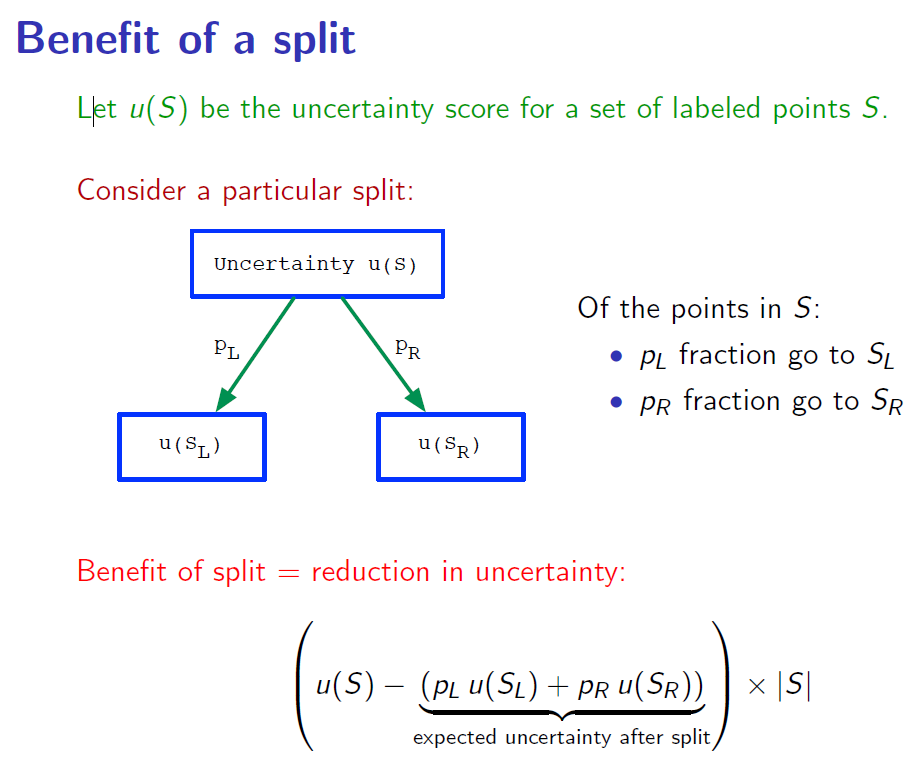
\includegraphics[width = 0.9\textwidth]{./images/feb/dt_split.PNG}
	}
	\label{fig:feb-dt-split}
	\caption{Benefit of a split.}
\end{figure} 


\textbf{When to stop?}\hspace{0.2cm} Keep splitting until leaves are pure. 

\textbf{Pruning.}\hspace{0.2cm} After split stops, we do pruning to avoid over-fitting. Consider all pairs of leave nodes,
any pair whose elimination yields a satisfactory (small)
increase in impurity is eliminated, and the common
antecedent node is declared as leaf node.

\subsection{Classification with generative models}

\textbf{Bayes-optimal prediction.}\hspace{0.2cm}
\begin{align}
	\begin{split}
	Pr(y= j | x) &= \frac{Pr(y= j) Pr(x|y=j)}{Pr(x)} \\
		&= \frac{\pi_j P_j(x)}{\sum_{i=1}^{k} \pi_i P_i(x)}
	\end{split}
\end{align}


\textbf{Laplace smoothing.}\hspace{0.2cm}
We want to estimate $p_{ji} = Pr(x_i = 1 | y=j)$. Then the maximum likelihood estimate of $p_{ji}$ is $p_{ij} = \frac{n_{ji}}{n_j}$, where $n_{ji}$ is the number of instances of class $j$ with $x_i = 1$, and $n_j$ is the number of 
instances of class $j$. 
\begin{remark}
This causes the problem if $n_{ji} = 0$. Instead, we use \textit{Laplace smoothing}: $p_{ji} = \frac{n_{ji} + 1}{n_j + 2}$
\end{remark} 


\textbf{Multinomial naive Bayes.}\hspace{0.2cm}
Classify document $x$ as $\argmax_j \pi_j \prod_{i=1}^{N} p_{ji} ^ {x_i}$.
To improve the performance, we may adopt the following heuristics:
\begin{itemize}
	\item Compensating for burstiness. Problem: once a word has appeared in a document, it has a much higher chance of appearing again.
	Solution: Instead of the number of occurrences $f$ of a word, use
	$\log(1 + f )$.
	
	\item Downweighting common words. Problem: common words can have a unduly large influence on classification. Solution: weight each word $w$ by \textit{inverse document frequency}:
	\[
		\log\frac{\# \text{docs}}{\#(\text{docs containing w})}
	\]
\end{itemize}

\subsection{Gaussian}
\textbf{Multivariate Gaussian.}\hspace{0.2cm} mean: $\mu \in R^p$. covariance $p\times p$
matrix $\sum$:
\begin{align}
\begin{split}
	p(x) &= \frac{1}{(2\pi)^{p/2} |\sum|^{1/2}} \exp(-\frac{1}{2} (x-\mu)^T \sum {}^{-1} (x-\mu))
\end{split}
\end{align}

\textbf{Spherical Gaussian.}\hspace{0.2cm} $\sum = diag(\sigma^2, ..., \sigma^2)$

\textbf{Diagonal Gaussian.}\hspace{0.2cm} $\sum = diag(\sigma_1^2, ..., \sigma_p^2)$





















% \chapter{March}

\section{Perceptron algorithm} \index{Perceptron algorithm}
Suppose we have input data $(x_1, y_1), (x_2, y_2), ..., (x_n, y_n) \in \mathbb{R}^p \times \{-1, 1\}$, 
and if the data points are separable, the perceptron algorithm works as following:

\begin{minted}[frame=lines, framesep=2mm,tabsize=4]{cpp}
w = 0
while some (x, y) is misclassified:
    w = w + yx
\end{minted}

\begin{remark}
In the separable case, perceptron algorithm guarantees to converge.
\end{remark}

\myheader{Multi-class perceptron}
\begin{minted}[frame=lines, framesep=2mm,tabsize=4]{cpp}
w_1 = w_2 = ... = w_k = 0
while some (x, y) is misclassified:
    for correct label y: w_y = w_y + x
    for incorrect label y*: w_(y*)  = w_(y*) - x
\end{minted}

\section{Kernel function} \index{Kernel function}
Following the perceptron algorithm, suppose $\phi$ is a function that maps $x$ to another feature space, such as $\phi(x) = (1, x_1, x_2, ..., x_1^2, x_2^2,..., x_1 x_2,...)$, which is a quadratic embedding.
In this case we can also run perceptron algorithm in the new feature space. 

\begin{minted}[frame=lines, framesep=2mm,tabsize=4]{cpp}
w = 0
while y*(w * \phi(x)) < 0:
w = w + y\phi(x)
\end{minted}

A problem is that every time we need to calculate $\phi(x)$, which may be of high dimensions. To solve this problem, we observe that in fact we don't need to access $\phi(x)$ at all to make a decision, instead we
can write $w$ as following:
\myequ{
    w = a_1 \phi(x_1) + a_2 \phi(x_2) + ... + a_n \phi(x_n)
}
then $w\cdot\phi(x)$ is a weighted sum of $\phi(x)\cdot\phi(x_i)$. In addition, we also observe that
\myequ{
    \phi(x) \cdot \phi(z) = (1 + x\cdot z)^2
}
That is, we don't need to calculate $\phi(x)$.


\myheader{kernel function} From above we know that we don't care about the embedding $\phi(x)$, we only 
care about the similarity between a pair of data points. Therefore, the kernel function is defined as following:
\vspace{0.5cm}
\begin{definition}[Kernel function]
    A function $k$: $\mathbb{R}^p \times \mathbb{R}^p \rightarrow \mathbb{R}$ is a valid kernel if it corresponds to some embedding, that is, there exists $\phi$ defined on $\mathbb{R}^p$ such that
    \myequ{
        k(x,z) = \phi(x) \cdot \phi(z)
        }
\end{definition}

This is equivalent to require that for any finite subset $\{x_1, x_2, ..., x_m\} \subset \mathbb{R}^p$,
the $m \times m$ similarity matrix 
\myequ{
    K_{ij} = k(x_i, x_j)
    }
is \textit{positive semidefinite}. Proof:
\myequ{
    Z^T K Z = Z^T (X^T X) Z = (XZ)^T (XZ) \geq 0
    }

\myheader{RBF kernel}
RBF kernel or Gaussian kernel is defined as
\myequ{
    k(x,z) = e^{-||x-z||^2 / 2\sigma^2}
    }

\myheader{string kernel}
For each substring $s$, we define feature:
\myequ{
    \phi_s(x) &= \# \text{ of times substring $s$ appears in $x$} \\
    \phi(x) &= (\phi_s(x): \text{ all strings } s)
    }


\section{$k$-means Clustering}\index{$k$-means Clustering}
\myheader{$k$-means} Minimize average squared distance between points and their nearest representatives.
The input is data points $x_1, x_2, ..., x_n$, and integer $k$, and the output is centers
$\mu_1, \mu_2, ..., \mu_k$.

\myheader{Lloyd's $k$-means algorithm}
\begin{minted}[frame=lines, framesep=2mm,tabsize=4]{cpp}
Initialize centers u_1, u_2, ... u_k in some manner.
Repeat until convergence:
    assign each point to its nearest center
    update each u_j to the mean of points assigned to it
\end{minted}

\myheader{How to initialize centers?} $k$-means++: start with extra centers, then prune later.

\begin{lstlisting}[
style=liststy,
]
Pick a data point x at random as the first center
Let $C = \{x\}$
    Repeat until the desired number of centers is attained:
    pick a data point $x$ at random from the following distributions: 
        $Pr(x) \propto dist(x, C)^2$, where $dist(x, C) = min_{z\in C}||x-z||$
    Add $x$ to $C$
\end{lstlisting}

\myheader{Streaming and online computation} If there are too much data to fit in memory, or the data
is continuously collected, we have to update the model gradually.

\myheader{The good and the bad} Good: fast and easy, effective in quantization. Bad: geared towards data in which the clusters are spherical, and of roughly the same results.

\section{Mixtures of Gaussians} \index{Mixtures of Gaussians}
Each of $k$ clusters is specified by a Guassian distribution $P_j = N(\mu_i, \sum_i)$ and a mixing weight
$\pi_j$. The overall distribution is a mixture of all Gaussians:
\myequ{
    Pr(x) = \pi_1 P_1(x) + \pi_2 P_2(x) + ... + \pi_k P_k(x)
}
We need to determine all the parameters including $\pi, \mu, \sum$. We apply \textbf{EM} algorithm to solve this problem
(see Figure~\ref{fig:em_mar}).
\begin{figure}[H]
    \centering{
        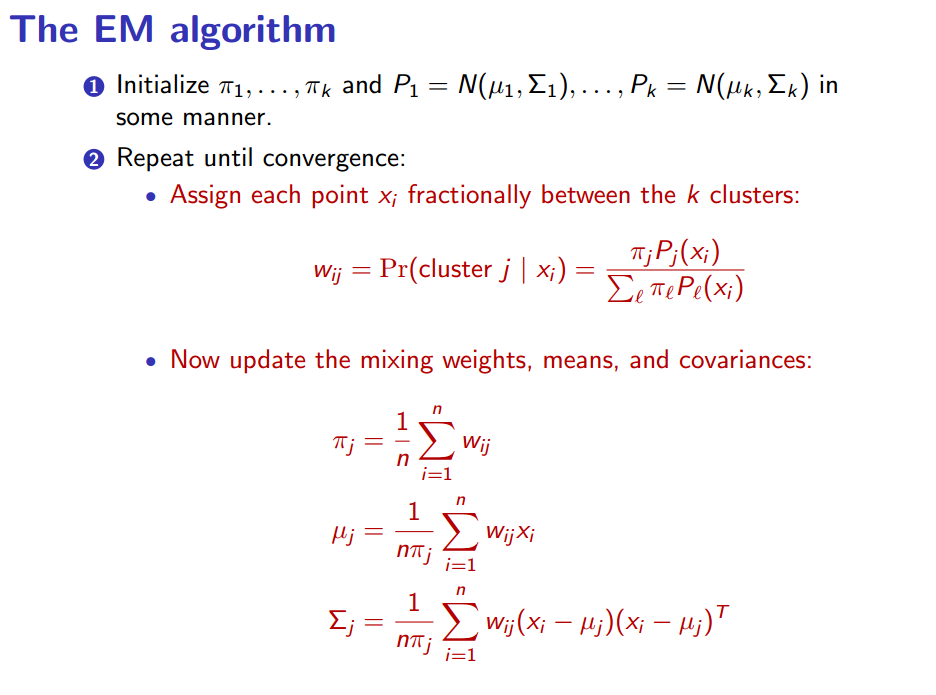
\includegraphics[width=0.9\textwidth]{./images/mar/gmm_em.PNG}
    }
    \caption{EM algorithm for GMM clustering.}
    \label{fig:em_mar}
\end{figure}

\section{Hierarchical clustering} \index{Hierarchical clustering}
Clustering is of multi-scale, and often there is no single right answer. Hierarchical 
clustering avoids these problems.
\begin{lstlisting}[
style=liststy,
]
Start with each point on its own
Repeat until there is just one cluster:
    Merge the two clusters with the $closest$ pair of points
Discard singleton clusters
\end{lstlisting}

\myheader{Linkage method} The problem is how we measure the distance
between two cluster of points.
\begin{enumerate}
    \item Single linkage: $dist(C, C') = min_{x \in C, x' \in C'} ||x - x'||$
    \item Complete linkage: $dist(C, C') = max_{x \in C, x' \in C'} ||x - x'||$
    \item Average linkage:
        \begin{enumerate}
            \item average pairwise distance between all pair of points in the two clusters
            \item distance between cluster centers
            \item Ward's method
        \end{enumerate}
\end{enumerate}


\section{Boosting}
\myheader{Adaboost} See Figure~\ref{fig:adaboost_mar}.
\begin{figure}[H]
    \centering{
        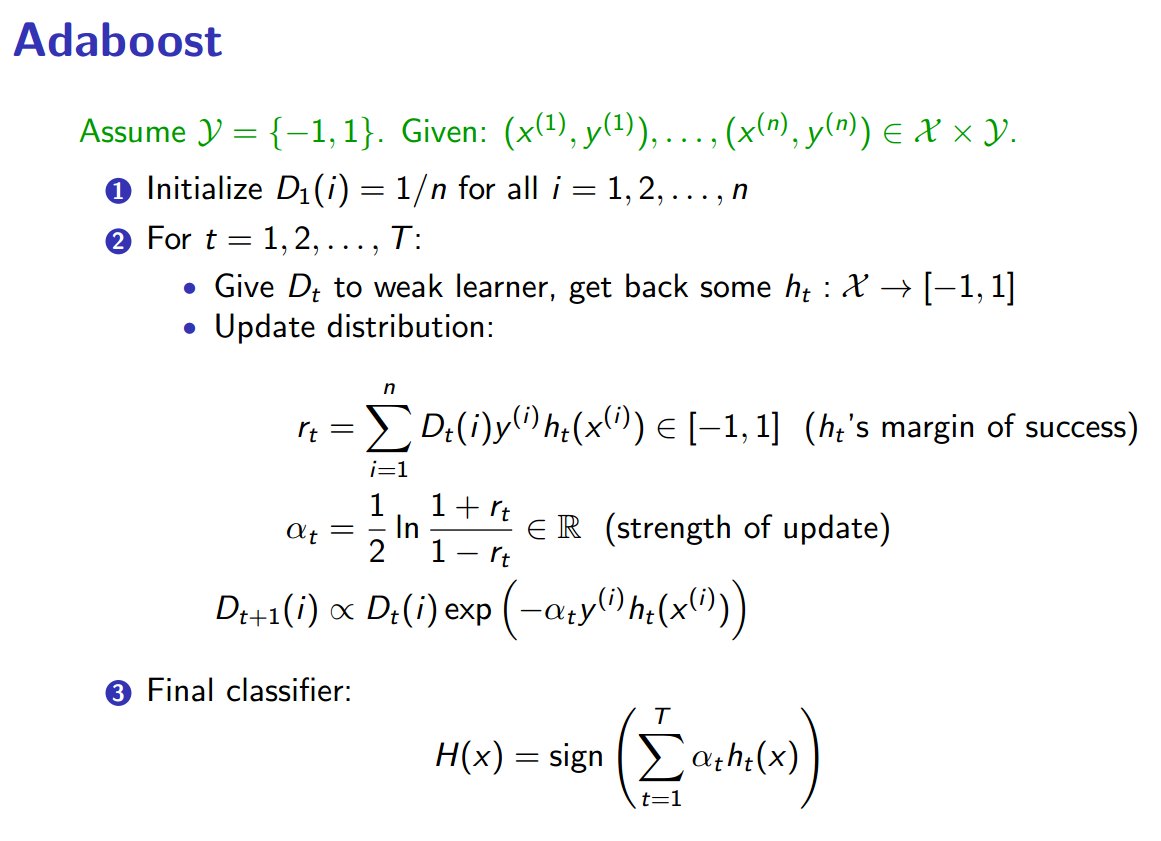
\includegraphics[width=0.9\textwidth]{./images/mar/adaboost.PNG}
    }
    \caption{Adaboost algorithms.}
    \label{fig:adaboost_mar}
\end{figure}

\myheader{Bagging} See Figure~\ref{fig:bagging_mar}
\begin{figure}[H]
    \centering{
        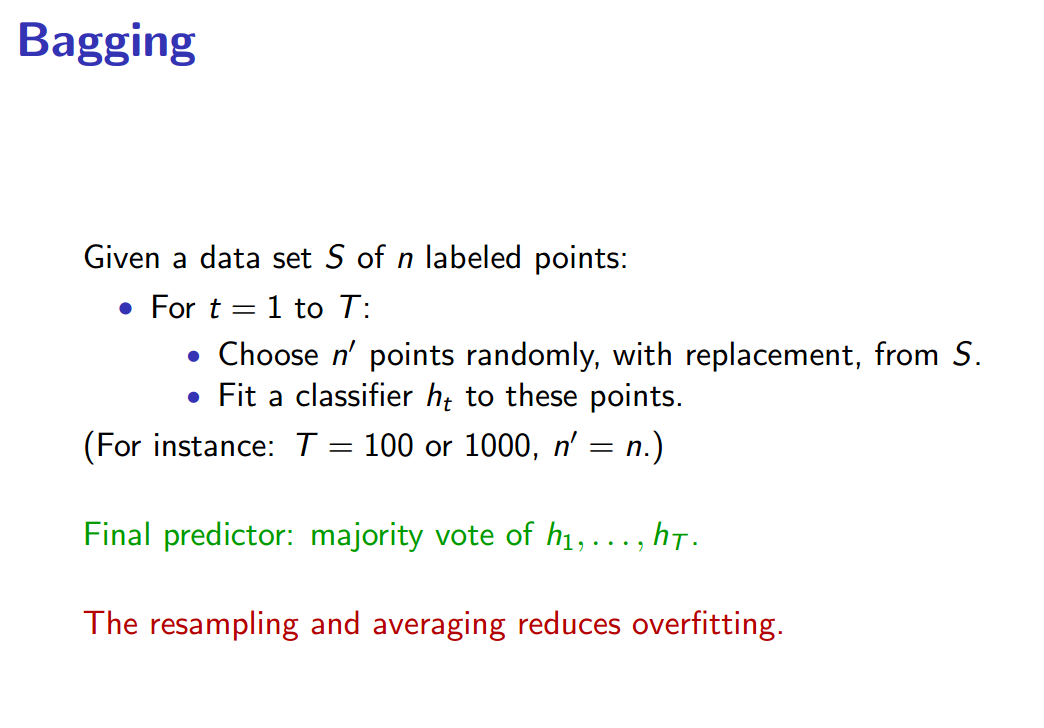
\includegraphics[width=0.9\textwidth]{./images/mar/bagging.PNG}
    }
    \caption{Bagging.}
    \label{fig:bagging_mar}
\end{figure}


\myheader{Random forest} See Figure~\ref{fig:random_forest_mar}
\begin{figure}[H]
    \centering{
        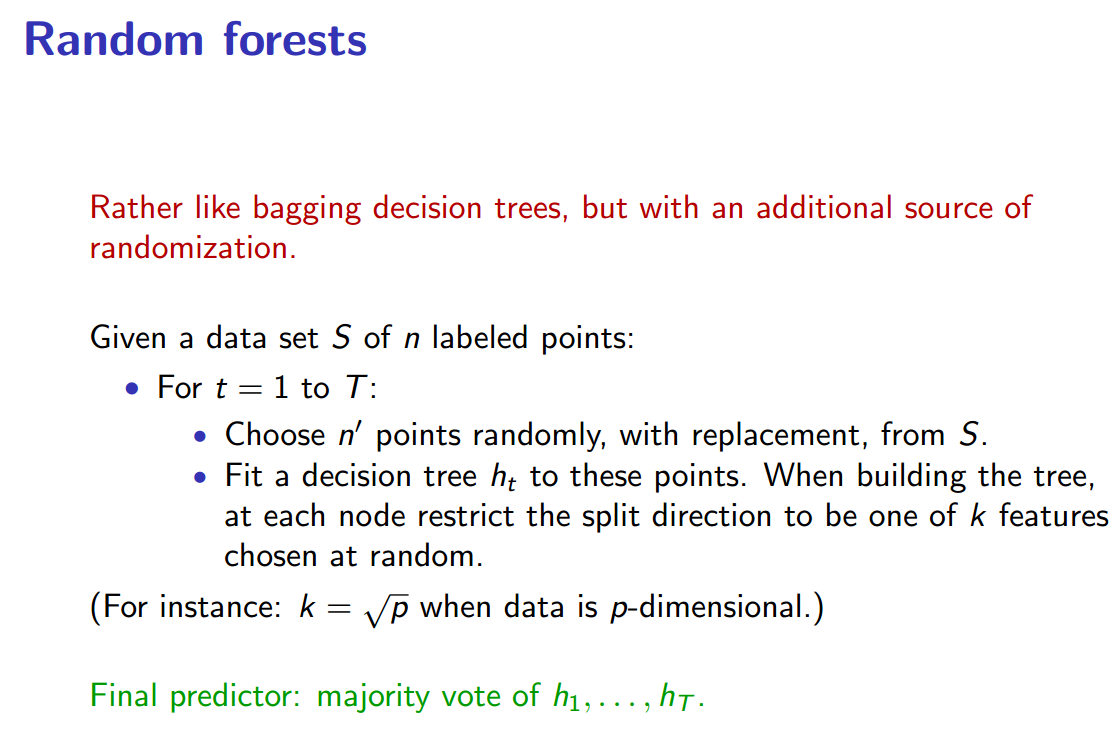
\includegraphics[width=0.9\textwidth]{./images/mar/random_forest.PNG}
    }
    \caption{Random forests.}
    \label{fig:random_forest_mar}
\end{figure}

\section{Informative projections} \index{Informative projections}

\myheader{Project to multiple directions} Suppose we want to project $x \in \mathbb{R}^p$
into the $k$-dimensional subspace spanned by $u_1, u_2, ..., u_k \in \mathbb{R}^p$, 
and suppose all $u_i$ are orthonormal (each has length one, and they are perpendicular to 
each other). Then the projection is:
\myequ{
    (x \cdot u_1)u_1 + (x \cdot u_2)u_2 + ... + (x \cdot u_k)u_k = UU^Tx
}

\myheader{Best single direction} Suppose we want to map our data $x_1, x_2, ..., x_n \in 
\mathbb{R}^p$ into just one dimension $x \mapsto u \cdot x$, what is the best direction $u$.

The best direction $u$ should be the one that maximize the variance after projection. Let $X$
be the data matrix, where each column is a data point, and $\sum$ be the covariance matrix of $X$. 
Suppose the mean of $X$ is $\mu \in \mathbb{R}^p$, then 
\myequ{
    \mathbb{E}(u^T X) & = u^T \mathbb{E}(X) = u^T \mu \\
    var(u^T X) & = \mathbb{E}(u^T X - u^T \mu) = \mathbb{E} (u^T (X - \mu) (X - \mu)^T u)  \\   
                & = u^T \mathbb{E}(X - \mu)(X - \mu)^T u = u^T \sum u
}

\begin{remark}
    $u^T\sum u$ is maximized by setting $u$ to the first \textbf{eigenvector} of $\sum$. The maximum
    value is the corresponding eigenvalue.
\end{remark}


\myheader{Best $k$-dimensional projection} Let $\sum$ be the $p\times p$ covariance matrix of $X$. 
and $\lambda_1 \geq  \lambda_2 \geq ... \geq \lambda_p$ are the eigenvalues, and $u_1, u_2, ...
u_p$ are the corresponding eigenvectors. Then the best $k$-dimensional projection directions are
$u_1, u_2, ..., u_k$.


\myheader{Spectral decomposition} See Figure~\ref{fig:spec_decomp_mar}.
\begin{figure}[H]
    \centering{
        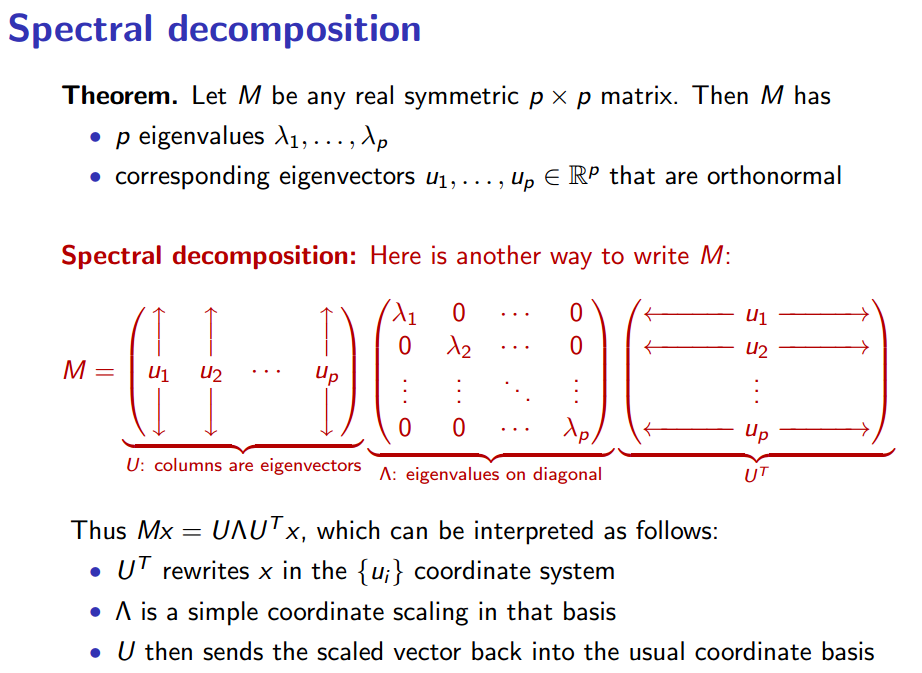
\includegraphics[width=0.9\textwidth]{./images/mar/spectral_decomp.PNG}
    }
    \caption{Spectral decomposition.}
    \label{fig:spec_decomp_mar}
\end{figure}

\myheader{Singular value decomposition (SVD)} See Figure~\ref{fig:svd_mar}. 
    Where $u_i, \sigma_i, v_i$ comes from? We know that:
    \begin{itemize}
        \item $Mv_i = \sigma_i u_i, M^T u_i = \sigma_i v_i$
        \item $M M^T u_i = \sigma_i^2 u_i, M^T M v_i = \sigma_i^2 v_i$
    \end{itemize}
    Therefore, $v_i$ is the eigenvectors of $M^T M$, and $u_i$ is the eigenvectors
    of $M M^T$. $MM^T$ and $M^TM$ has the same eigenvalues $\sigma_i^2$.  Note
    that all $\sigma_i$ are \textbf{non-negative}.

\begin{figure}[H]
    \centering{
        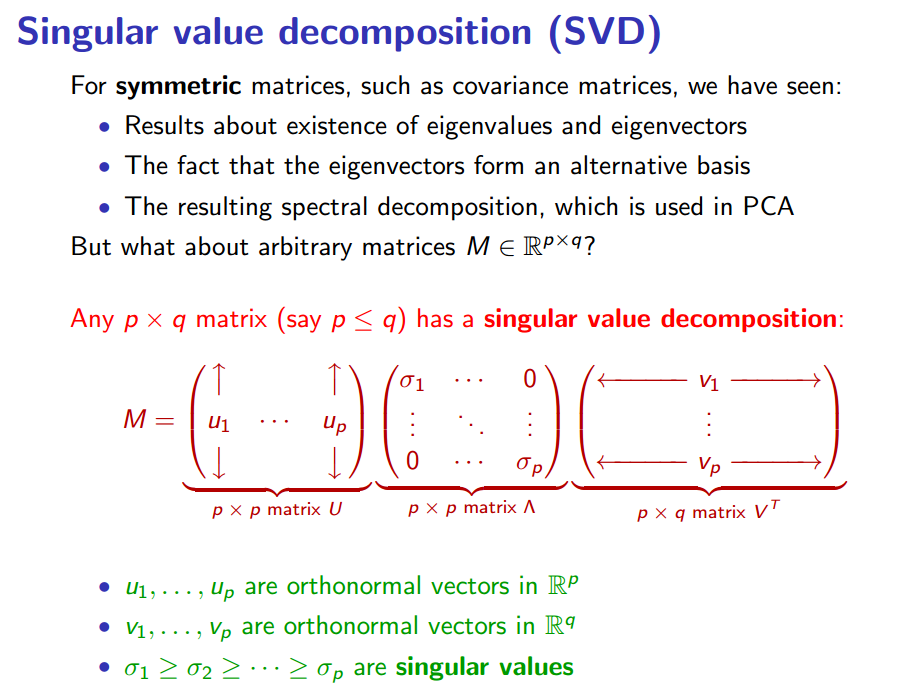
\includegraphics[width=0.9\textwidth]{./images/mar/SVD.PNG}
    }
    \caption{Singular value decomposition.}
    \label{fig:svd_mar}
\end{figure}

\section{Positive definite matrix }
\vspace{0.5cm}
\begin{definition}[Positive definite matrix]
    A square $p \times p$ symmetric matrix $A$ is positive definite if for all
    nonzero $x \in \mathbb{R}^p$,
    \myequ{
        x^T A x > 0
        }
\end{definition}

\myheader{Properties of positive definite matrix}
\begin{enumerate}
    \item The $r \times r$ submatrix $A_r$ (start from top left element) is also positive
    semidefinite.
    \item The $p$ eigenvalues of A $\lambda_1, \lambda_2, ..., \lambda_p$ are positive.
    Conversely, if all the eigenvalues of a matrix $B$ are
    positive, then $B$ is positive definite.
    
    \item There exist a unique decomposition of $A = LL^T$, where $L$ is a lower triangular
    matrix. This is called \textit{Cholesky Decomposition}. 
    \item There exists a unique decomposition of $A = VDV^T$.
    
\end{enumerate}
        
  

\section{Beyond projections} \index{Beyond projections}
Sometimes data in a high-dimensional space $\mathbb{R}^p$ in fact
lies close to a $k$-dimensional manifold, for $k\ll p$.

\myheader{ISOMAP algorithm}
Given data $x_1, x_2, ..., x_n$,
\begin{enumerate}
\item estimate \textit{geodesic distances} between the data points, that is, distance along the manifold.
\item embed these points in Euclidean space so as to match these distances.
\end{enumerate}

\myheader{Geodesic distances}
To estimate geodesic distances:
\begin{enumerate}
   \item Construct neighborhood graph, connect nodes whenever two nodes are close together.
   \item Compute distance in this graph (shortest-path algorithm).  
\end{enumerate}

\myheader{Distance-preserving embeddings} Problem definition:
\begin{lstlisting}[
style=liststy,] 
Input:an $n\times n$ matrix of pairwise distances $D$, where $D_ij$ is the distance between 
points $i$ and $j$.
Output: an embedding $z_1, z_2, ..., z_n \in \mathbb{R}^k$ that realizes these distances as closely as 
possible.
\end{lstlisting}

\myheader{Gram matrix}
Gram matrix on a set of vectors $z_1, z_2, ..., z_n$ is the matrix $B$ where
$B_{ij} = z_i \cdot z_j$.

\myheader{Classical multidimensional scaling} See Figure~\ref{fig:cms_mar}

\begin{figure}[H]
    \centering{
        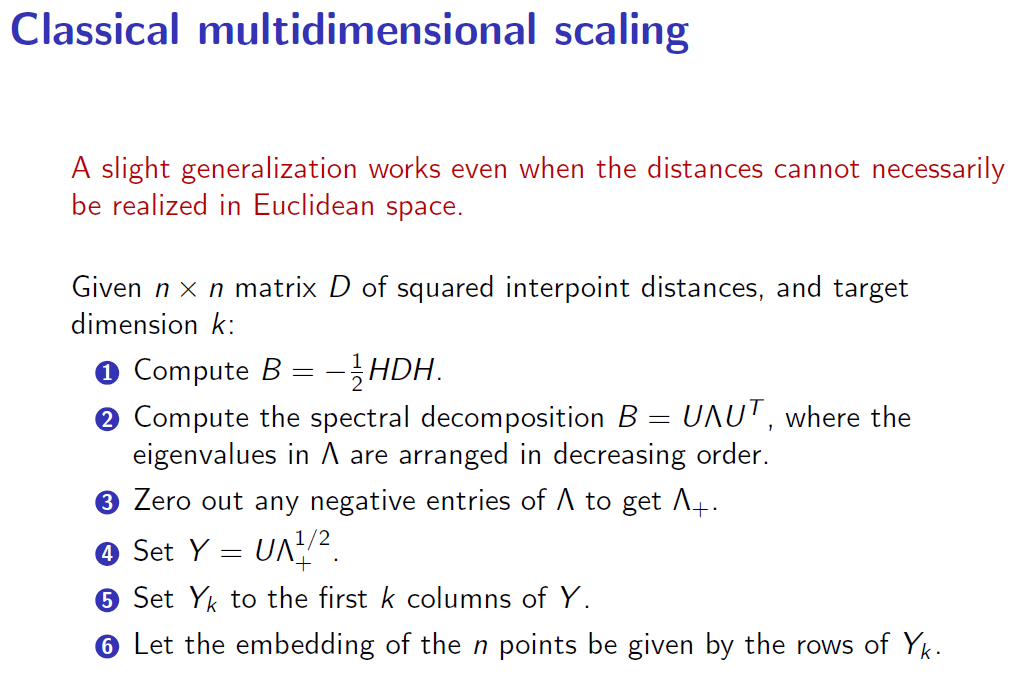
\includegraphics[width=0.9\textwidth]{./images/mar/cms.PNG}
    }
    \caption{Classical multidimensional scaling.}
    \label{fig:cms_mar}
\end{figure}


\section{Jacobian matrix} \index{Jacobian matrix}
In vector calculus, the Jacobian matrix is the matrix of all first-order partial derivatives of a vector-valued function.
\myequ{
    J  = \frac{d \mathbf{f}}{d \mathbf{x}} &= \begin{bmatrix}
        \frac{\partial \mathbf{f}}{\partial x_1} &
         \frac{\partial \mathbf{f}}{\partial x_2} &
         \dots & \frac{\partial \mathbf{f}}{\partial x_n} 
    \end{bmatrix}    \\
    & = \begin{bmatrix}
        \frac{\partial f_1}{\partial x_1} &
        \dots &
        \frac{\partial f_1}{\partial x_n} \\
         \vdots & \ddots & \vdots \\
         \frac{\partial f_m}{\partial x_1}  &
         \dots &
         \frac{\partial f_m}{\partial x_n} 
    \end{bmatrix}
}

\section{Gaussian-Newton algorithm} \index{Gaussian-Newton algorithm}
The Gaussian-Newton algorithm is used to solve non-linear least square problems. It is a modification
of Newton's method for finding a minimum of a function. Unlike Newton's method, the Gaussian-Newton algorithm
can only be used to minimize a sum of squared function values, but it has the advantage that the second
derivatives, which can be challenging to compute, are not required.

Given $m$ functions $r = (r_1, r_2, \dots, r_m)$ (often called residuals) of $n$ variables $\mathbf{\beta} = (\beta_1, \dots, \beta_n)$ with $m \geq n$, the Gauss–Newton algorithm iteratively finds the value of the variables which minimizes the sum of squares:
\myequ{
  S(\beta) = \sum\limits_{i=1}^{m} r_i^2(\beta)
} 
Start with an initial guess $\mathbf{\beta}^{(0)}$, the method proceeds by the iterations:
\myequ{
    \mathbf{\beta}^{(s+1)} = \mathbf{\beta}^{(s)}    - (J_r^T J_r)^{-1} J_r^T r(\mathbf{\beta}^{(s)})    
}
where 
\myequ{
    (J_r)_{ij} = \frac{\partial r_i(\beta^{(s)})}{\partial \beta_j}
}
If $m = n$, the iteration simplifies to 
\myequ{
    \mathbf{\beta}^{(s+1)} = \mathbf{\beta}^{(s)}    - (J_r)^{-1} r(\mathbf{\beta}^{(s)})
}


\section{Functional programming: introductions} \index{Functional programming: introductions}

\myheader{Why FP?}
We want software to be \textit{readable, reusable, modifiable, predictable and checkable}. Functional
programming could satisfy these requirements. 

There is no assignment, mutation, or loop in FP.

\section{$\lambda$-calculus}\index{$\lambda$-calculus}
Lambda calculus (also written as $\lambda$-calculus) is a formal system in mathematical logic for expressing computation
 based on function abstraction and application using variable binding and substitution.

\myheader{Syntax}
Three kinds of expressions:
\begin{lstlisting}[
style=liststy,] 
e ::= x             
    | $\lambda$ x. e      
    | $\lambda$ e_1 e_2   
\end{lstlisting}
called \textit{variables}, \textit{functions}($\lambda$-abstraction), and \textit{application}.
Functions $\lambda x. e$ takes $x$ as an input and output $e$.
 
Application associates to the left: $x y z$ means $(x y) z$. However, abstraction extends as far right
as possible:
$\lambda x. x \lambda y. x y z \Rightarrow \lambda x. (x \lambda y. ((x y) z))$ 

Identity function: $I = \lambda x. x$

\myheader{Scope of identifier (variable)}
Scope of a variable is the part of program where the variable is \textit{accessible}.

$\lambda x. E$ binds variable $x$ in $E$:
\begin{enumerate}
    \item $x$ is the newly introduced varialbe.
    \item $E$ is the scope of $x$.
    \item $x$ is bound in $\lambda x. E$
\end{enumerate}

$y$ is \textit{free} if it occurs not bound in $E$:
\begin{enumerate}
    \item $Free(x) = \{x\}$
    \item $Free(E_1 E_2) = Free(E_1) \cup Free(E_2)$ 
    \item $Free(\lambda x. E) = Free(E) - \{x\}$
\end{enumerate}

$\alpha$-renaming:
\begin{enumerate}
    \item Allows bound variable names to be changed.
    \item $\lambda x. x = \lambda y. y$
\end{enumerate}

substitution:
\begin{enumerate}
    \item $[E'/x]E$: use $E'$ to substitute all $x$ bounded in $E$
    \item $[y (\lambda x. x)/x] \lambda y. (\lambda x. x) y x
           \equiv$
           $[y (\lambda v. v)/x] \lambda y. (\lambda u. u) z x $ (renaming)
           $\equiv \lambda z. (\lambda u. u) z (y (\lambda v. v))$ (substitution) 
\end{enumerate}

$\beta$-reduction:
\begin{enumerate}
    \item $\beta$-reduction captures the idea of function application.
    \item $(\lambda x. e) e' \rightarrow [e'/x]e$
    \item $((\lambda n. n\times2) 7) \rightarrow 7\times 2$
\end{enumerate}

local variable:
\begin{lstlisting}[
style=liststy,] 
let x = $e_1$ in $e_2$
$\equiv (\lambda x. e_2) e_1$
\end{lstlisting}

boolean:
\begin{lstlisting}[
style=liststy,] 
true $\equiv$ $\lambda x. \lambda y. x$
false $\equiv$ $\lambda x. \lambda y. y$
if $E_1$ then $E_2$ else $E_3$ $\equiv$ $E_1 E_2 E_3$
if true then u else v $\rightarrow$ $(\lambda x. \lambda y. x) u\ v  \rightarrow (\lambda  y. u) \rightarrow u$  
\end{lstlisting}

not:
\begin{lstlisting}[
style=liststy,]
function takes b:
    return function x, y:
        return (if b then y else x)

not $\equiv \lambda b. (\lambda x. \lambda y. \  b\ y\ x)$
not true $\rightarrow \lambda x. \lambda y. \ true \ y \ x \rightarrow \lambda x. \lambda y. \ y \rightarrow false$ 
\end{lstlisting}

or:
\begin{lstlisting}[
style=liststy,] 
function takes $b_1, b_2$
    return function takes x, y:
        return (if $b_1$ then x else (if $b_2$ then x else y))
or $\equiv \lambda b_1 . \lambda b_2 . (\lambda x. \lambda y.\ b_1\ x (b_2 \ x \ y))$  
\end{lstlisting}

records:
\begin{lstlisting}[
style=liststy,] 
pair = function takes a bool
       return the left or right element
mkpair $e_1 \ e_2 \equiv \lambda b. \ b\ e_1\ e_2$  
fst p $\equiv$ p true
snd p $\equiv$ p false
\end{lstlisting}

natural numbers:
\begin{lstlisting}[
style=liststy,] 
natural number: iterate a number of times over some function
$n$ = function that takes function $f$, starting value $s$
      returns: $f$ applied to $s$ $n$ times
$0 \equiv \lambda f. \lambda s. \ s$
$1 \equiv \lambda f. \lambda s. \ f \ s$
$2 \equiv \lambda f. \lambda s. \ f (f \ s)$
(n f s) = apply f to s n times
\end{lstlisting}

operations on natural numbers:
\begin{lstlisting}[
style=liststy,] 
iszero n $\Leftrightarrow$ n ($\lambda$ b. false) true
iszero $\Leftrightarrow$ $\lambda $ n. ($\lambda$ b. false) true
succ n  $\Leftrightarrow$ $\lambda$f. $\lambda$s. f (n f s)
add a b $\Leftrightarrow$ a succ b
multi a b $\Leftrightarrow$ a (add b) 0
\end{lstlisting}


\section{Haskell: basics}\index{Haskell: basics}
Haskell is a standardized, general-purpose purely functional programming language, with non-strict semantics and strong static typing.

\myheader{GHC system}
\begin{lstlisting}[
style=liststy,
language=Haskell,]
:load foo.hs
:type expression
:info variable
\end{lstlisting}

\myheader{Basic types}
\begin{haskellcode}
32   :: Integer
4.2  :: Double
'a'  :: Char
True :: Bool

-- function types
pos :: Integer -> Bool
pos x = (x > 0)

-- multiple argument function types
-- function takes args of A1, A2, A3, gives out B
A1 -> A2 -> A3 -> B

-- tuples, elements do not have to be of the same type
(A1, ..., An)
-- pattern matching extracts values from tuple
pat :: (Int, Int, Int) -> Int
pat (x, y, z) = x * (y + z)

-- Lists, elements have to be of the same type
[1, 3, 5, 7]
-- construct lists
'a' : ['b', 'c'] = ['a', 'b', 'c']
cons2 x y zs = x : y : zs

-- type
-- Not a new type, just shorthand
type XY = (Double, Double)
type Circle = (Double, Double, Double)
-- data creates new types
data CircleT = Circle (Double, Double, Double)
data Shape =
    | Rectangle Side Side
    | Ellipse Radius Radius
    | RtTriangle Side Side
    | Polygon [Vertex]
type Side = Double
type Radius = Double
type Vertex = (Double, Double)
\end{haskellcode}


\myheader{Input and output}

\begin{haskellcode}
-- action: value describing an effect on world
IO a -- type of an action that returns an a

-- takes input string, return action that writes string to stdout
putStr :: String -> IO () 

-- only one way to execute action: make it the value of name main
main :: IO ()
main = putStr "hello world\n"

-- do many actions with 'do'
do putStr "Hello"
   putStr "World"
   putStr "\n"
   
-- input
getLine :: IO String
main:: IO()
main = do putStr "What is your name?"
       n <- getLine -- assignment
       putStrLn ("Happy New Year " ++ n)
\end{haskellcode}


\section{Haskell: higher-order functions}\index{Haskell: higher-order functions}
In all functional languages, functions are first-class values, meaning, that they can be treated just as you would any other data. That is, you can pass functions around to in any manner that you can pass any other data around in.

\myheader{Functions are data}
\begin{haskellcode}
plus1 :: Int -> Int
plus1 x = x + 1

minus1 :: Int -> Int
minus1 x = x - 1

funp :: (Int -> Int, Int -> Int)
funp = (plus1, minus1)
\end{haskellcode}

\myheader{Take functions as input and output}
\begin{haskellcode}
-- functions as input
doTwice :: (t -> t) -> t -> t
doTwice f x = f (f x)

-- functions as output
plusn :: Int -> (Int -> Int)
plusn n = f
          where f x = x + n

-- partially apply functions
plus :: Int -> Int -> Int
plus a b = a + b
plus5 :: Int -> Int
plus5 = plus 5 -- plus5 1000 outputs 1005
\end{haskellcode}

\myheader{Anonymous functions}
We will see many situations where a particular function is only used once, and hence, 
there is no need to explicitly name it. Haskell provides a mechanism to create such anonymous functions.

\begin{haskellcode}
\x -> x + 1
(\x -> x + 1) 100 -- 101
doTwice (\x -> x + 1) 100 -- 102
\end{haskellcode}

\myheader{Infix operations}
Haskell allows you to use any function as an infix operator,
simply by wrapping it inside backticks.

To further improve readability, Haskell allows you to use partially applied infix operators, ie infix operators with only a single argument. These are called \textit{sections}.
\begin{haskellcode}
2 `plus` 4 -- 6
doTwice (+1) 0 -- 2
doTwice (1+) 0 -- 2
doTwice (1:) [2..5] -- [1, 1, 2, 3, 4, 5]
\end{haskellcode}

\myheader{Polymorphism}
\textit{doTwice} is polymorphic in that it works with different kinds of values, 
e.g. functions that increment integers and concatenate strings. This is vital for \textit{abstraction}.

Polymorphic functions which can operate on different kinds values are often associated with polymorphic 
data structures which can contain different kinds of values. 
These are also represented by types containing type variables.

\begin{haskellcode}
foo :: a -> (a -> b) -> b
foo x f = f x

x |> f = f x

do1 :: (a -> b) -> a -> b
do1 f x = x |> f

do2 :: (a -> a) -> a -> a
do2 f x = x |> f |> f
\end{haskellcode}

\myheader{Bottling Computation Patterns With Polymorphic Higher-Order Functions}

\begin{haskellcode}
toUpperString :: String -> String
toUpperString [] = []
toUpperString (c:cs) = toUpper c : toUpperString cs

-- map
map :: (a -> b) -> [a] -> [b]
map f [] = []
map f (x:xs) = (f x) : (map f xs)

toUpperString = map toUpper

-- foldr
foldr op base [] = base
foldr op base (x:xs) = x `op` (foldr op base xs)

-- foldr on actions
fuseActions :: [IO ()] -> IO ()
fuseActions []        = return ()
fuseActions (a1:acts) = do a1
                           fuseActions acts

fuseActions :: [IO ()] -> IO ()
fuseActions = foldr (>>) (return ())
\end{haskellcode}

\section{Higher-order programming} \index{Higher-order programming}

\myheader{Recursive types}
\begin{haskellcode}
data Shape  = Rectangle Double Double 
            | Polygon [(Double, Double)]

data IntTree = ILeaf Int
             | INode IntTree IntTree
\end{haskellcode}

\myheader{Parameterized types}

\begin{haskellcode}
-- a is a type
data List a = Empty
            | OneAndMore a (List a)

data Tree a = Leaf a
            | Node (Tree a) (Tree a)

type IntList = List Int
type CharList = List Char
type DoubleList = List Double
\end{haskellcode}

\myheader{Kinds}
In the area of mathematical logic and computer science known as type theory, 
a kind is the type of a type constructor or, less commonly, the type of a higher-order type operator. 

The \textit{Tree a} corresponds to trees of values of type a. 
If a is the type parameter, then what is Tree ? 
A function that takes a type a as input and returns a type Tree a as output! 
But wait, if List is a function then what is its type? A \textit{kind} is the type of a type.

\begin{haskellcode}
:kind Int -- *
:kind Char -- *
:kind Bool -- * -> *
:kind (->) -- * -> * -> *
\end{haskellcode}

\begin{enumerate}
    \item *: the kind of all data types seen as nullary type constructors, 
    and also called proper types in this context.
    \item * -> * : the kind of a unary type constructor, e.g. list type constructor.
    \item * -> * -> * : the kind of a binary type constructor (via currying), e.g. of 
             a pair type constructor  and also that of a function type constructor.
    \item (* -> *) -> *: the kind of a higher-order type operator from unary type constructors to proper types.
\end{enumerate}


\section{Haskell: typeclass}\index{Haskell: typeclass}
We want the operator such as $+$ to work for a bunch of different data types
such as integers, doubles. So what should be the type of $+$?

\begin{haskellcode}
-- too anemic
(+) :: Integer -> Integer -> Integer
-- too aggressive, it doesn’t make sense to add two functions
(+) :: a -> a -> a
\end{haskellcode}

Haskell solves this problem with an insanely slick mechanism called typeclasses.

\myheader{Qualified types}
\begin{haskellcode}
-- truth
(+) :: (Num a) => a -> a -> a
\end{haskellcode}
We call the above a qualified type. Read it as, $+$ takes in two a values and returns an a value 
for any type a that is a Num or is an instance of Num.

The name Num can be thought of as a predicate over types. 
Some types satisfy the Num predicate. Examples include Integer, Double etc, and any values of those types can be passed to +. 
Other types do not satisfy the predicate. Examples include Char, String, functions etc, and 
so values of those types cannot be passed to +.

\myheader{Typeclass}
A \textit{typeclass} is a collection of operations (functions) that must exist for the underlying type.

A typeclass defines some behavior (like comparing for equality, comparing for ordering, enumeration) and then types that can behave in that way are made instances of that typeclass. The behavior of typeclasses is achieved by defining functions or just type declarations that we then implement. So when we say that a type is an instance of a typeclass, we mean that we can use the functions that the typeclass defines with that type.




\begin{haskellcode}
-- typeclass Eq
class  Eq a  where
  (==) :: a -> a -> Bool
  (/=) :: a -> a -> Bool

-- typeclass show
class  Show a  where
  show :: a -> String
\end{haskellcode}
A type a can be an instance of Eq as long as there are two functions 
that determine if two a values are respectively equal or disequal. 
Similarly, the typeclass Show captures the requirements that make a particular datatype be viewable,

\myheader{Automatic derivation}
Haskell allows us automatically derive functions for certain key type classes, namely those in the standard library.
\begin{haskellcode}
data Showable = A' | B' | C' deriving (Eq, Show)

class (Eq a, Show a) => Num a where
    (+) :: a -> a -> a
    (*) :: a -> a -> a
    (-) :: a -> a -> a
    negate :: a -> a
    abs :: a -> a
    signum :: a -> a
    fromInteger :: Integer -> a
-- A type T can only be deemed an instance of Num if
--     1. The type is also an instance of Eq and Show, and
--     2. There are functions for adding, multiplying, etc
\end{haskellcode}

\myheader{Explicit signatures}
While Haskell is pretty good about inferring types in general, 
there are cases when the use of type classes requires explicit annotations.
\begin{haskellcode}
-- Read is a build typeclass, parse a string and turn it into an a
read:: (Read a) => String -> a

-- read "2" -- error: it doesn’t know what to convert the string to
-- (read "2") :: Int -- correct
-- (read "2") :: Double -- correct
\end{haskellcode}


\section{Haskell: monads}\index{Haskell: monads}
The function programming community divides into two camps:
\begin{enumerate}
    \item "Pure" languages, such as Haskell, are based directly upon the 
    mathematical notion of a function as a mapping from arguments to 
    results.

    \item "Impure" languages, such as ML, are based upon the extension of this notion with a range of possible effects, such as exceptions and assignments.
\end{enumerate}
Pure languages are easier to reason about and may benefit from lazy
evaluation, while impure languages may be more efficient 
and can lead to shorter programs.

\subsection{Abstracting programming patterns}
Monads are an example of the idea of abstracting out a common 
programming pattern as a definition. 

\begin{haskellcode}
inc :: [Int] -> [Int]
inc []     =  []
inc (n:ns) =  n+1 : inc ns

sqr :: [Int] -> [Int]
sqr []     =  []
sqr (n:ns) =  n^2 : sqr ns

-- above functions have the same programming pattern, 
-- namely mapping the empty list to itself, and a non-empty 
-- list to some function applied to each element in the list

-- abstract this pattern gives us the map function
map         :: (a -> b) -> [a] -> [b]
map f []     = []
map f (x:xs) = f x : map f xs

inc = map (+1)
sqr = map (^2)
\end{haskellcode}

\myheader{Maybe}
The \texttt{Maybe} type encapsulates an optional value.
A value of type \texttt{Maybe a} either 
contains a value of type \texttt{a} (represented as \text{Just a}), 
or it is empty 
(represented as \texttt{Nothing}). 
Using \texttt{Maybe} is a good way to deal with errors or 
exceptional cases without resorting to drastic measures such as error.


\begin{haskellcode}
data Maybe a = Just a | Nothing

foo :: (a -> b) -> Maybe a -> Maybe b
foo f z = case z of 
            Just x  -> Just (f x)
            Nothing -> Nothing 
\end{haskellcode}

\myheader{Functor typeclass}
Functor typeclass is basically for things that can be mapped over. 
\begin{haskellcode}
class Functor f where  
    fmap :: (a -> b) -> f a -> f b

-- map is just a map that works on lists
instance Functor [] where
    fmap = map

-- Maybe is also a functor
instance Functor Maybe where
    fmap f (Just x) = Just (f x)
    fmap f Nothing = Nothing

-- make Tree type instance of Functor
instance Functor Tree where
    fmap f EmptyTree = EmptyTree
    fmap f (Node x left right) = Node (f x) 
           (fmap f left) (fmap f right)

-- IO is an instance of Functor
instance Functor IO where
    fmap f action = do
        results <- action
        return (f result)

-- <-: bind that result to a name
result <- getLine

-- return: a function that makes an I/O action that doesn't do 
--         anything but only presents something as its result

\end{haskellcode}


\myheader{Generalize map to many arguments}
We can generalize map to many arguments.
\begin{haskellcode}
lift1 :: (a -> b) -> [a] -> [b]
lift2 :: (a1 -> a2 -> b) -> [a1] -> [a2] -> [b]
lift3 :: (a1 -> a2 -> a3 -> b) -> [a1] -> [a2] -> [a3] -> [b]
\end{haskellcode}

There is a typeclass called \texttt{Applicative} that corresponds to 
the type constructors that you can \texttt{lift2} or \texttt{lift3} over.

\begin{haskellcode}
liftA  :: Applicative t => (a -> b) -> t a -> t b

liftA2 :: Applicative t 
       => (a1 -> a2 -> b) 
       -> t a1 
       -> t a2 
       -> t b

liftA3 :: Applicative t 
       => (a1 -> a2 -> a3 -> b) 
       -> t a1 
       -> t a2
       -> t a3
       -> t b
\end{haskellcode}   


\myheader{Sequencing operator}
Here we introduce a new sequencing operator that we write as 
\texttt{>>=}, and read as \textit{then}.

\begin{haskellcode}
(>>=)   :: Maybe a -> (a -> Maybe b) -> Maybe b
m >>= f =  case m of
             Nothing -> Nothing
             Just x  -> f x

-- evaluate each of the expression m1, m2, ..., mn in turn,
-- and combine their results x1, x2, ..., xn by applying 
-- the function f
m1 >>= \x1 ->
  m2 >>= \x2 ->
  ...
    mn >>= \xn ->
      f x1 x2 ... xn
\end{haskellcode}


\chapter{May}

\section{Build sparse matrix with Eigen efficiently} \index{Build sparse matrix with Eigen efficiently}

When I build a sparse matrix with Eigen, I come across a problem that it is quite slow. The problem is that
when you \textit{insert} elements one by one, each time Eigen needs to reallocate space for the matrix and copy
the data, which is reason that it can be slow. 

The solution is to first record the row, column index as well as value of non-zero entries with \textit{triplets},
and then build the sparse matrix with the function \textit{setFromTriplets}.

\chapter{June}
\section{Transform matrix and projective matrix} \index{Transform matrix and projective matrix}
To transform a vertex from world space to camera space, we need to construct the rigid transform matrix. Given a right
hand system, we need \textbf{eye} $\in \mathbb{R}^3$ position, \textbf{lookAt} $\in \mathbb{R}^3$ position as well as \textbf{up} $\in \mathbb{R}^3$ direction to determine the matrix.
The matrix is in the following format:
 \myequ{
V & =       \begin{pmatrix}
           s.x & u.x & -f.x & 0.0 \\
           s.y & u.y & -f.y & 0.0 \\
           s.z & u.z & -f.z & 0.0 \\
           - (s \cdot eye) & -(u \cdot eye) & -(f \cdot eye) & 1.0  
       \end{pmatrix} \\
  where\  & f = normalize(lookAt - eye) \\
  & s = normalize(f \times up) \\
  & u = s \times f 
}

\begin{remark}
    Note this matrix is constructed for right-hand coordinate system.  
\end{remark}

In addition, to transform a point from camera space to image space, we need to construct the perspective projection matrix. 
In this case, we need field of view in $x$ and $y$ axis, namely \textbf{fovX} and \textbf{fovY}, \textbf{nearClip} and \textbf{farClip}. The matrix is build as:
 
 \myequ{
     P & =       \begin{pmatrix}
        \frac{1}{\text{tan}(\frac{fovX}{2})} & 0 & 0 & 0 \\
        0 & \frac{1}{\text{tan}(\frac{fovY}{2})} & 0 & 0 \\
        0 & 0 & -\frac{far + near}{far - near} 
        &  -\frac{2 * far * near}{far - near} \\
        0 & 0 & -1 & 0 
 \end{pmatrix} 
}



















\end{document}